% \documentclass[sort&compress]{elsarticle}
\documentclass[final,3p,times,twocolumn,sort&compress]{elsarticle}
%\documentclass[review]{elsarticle}


\usepackage{lineno,hyperref}
\modulolinenumbers[2]

\journal{Remote Sensing of Environment}

%% Packages
\usepackage{tabu}
\usepackage{breakurl}
\usepackage{float}

%%%%%%%%%%%%%%%%%%%%%%%
%% Elsevier bibliography styles
%%%%%%%%%%%%%%%%%%%%%%%
%% To change the style, put a % in front of the second line of the current style and
%% remove the % from the second line of the style you would like to use.
%%%%%%%%%%%%%%%%%%%%%%%

%% Numbered
% \bibliographystyle{model1-num-names}

%% Numbered without titles
%\bibliographystyle{model1a-num-names}

%% Harvard
% \bibliographystyle{model2-names.bst}\biboptions{authoryear}

%% Vancouver numbered
% \usepackage{numcompress}\bibliographystyle{model3-num-names}

%% Vancouver name/year
% \usepackage{numcompress}\bibliographystyle{model4-names}\biboptions{authoryear}

%% APA style
%\bibliographystyle{model5-names}\biboptions{authoryear}

%% AMA style
% \usepackage{numcompress}
% \bibliographystyle{model6-num-names}

%% `Elsevier LaTeX' style
\bibliographystyle{elsarticle-num}

%%%%%%%%%%%%%%%%%%%%%%%

\begin{document}

\begin{frontmatter}

\title{Night and day: What are the nonlinear associations between urban characteristics and land surface temperature?}

%% or include affiliations in footnotes:
\author[1]{T.M. Logan\corref{mycorrespondingauthor}}
\cortext[mycorrespondingauthor]{Corresponding author}
% \ead[url]{www.tomlogan.co.nz}
\ead{tom.logan@canterbury.ac.nz}

\author[2]{B. Zaitchik}
\author[1]{S. Guikema}


\address[1]{Industrial and Operations Engineering, University of Michigan, Ann Arbor, MI}
\address[2]{Earth and Planetary Sciences, Johns Hopkins University, Baltimore, MD}

\begin{abstract}
Although heat waves and the urban heat island are nocturnal phenomena, the drivers of land surface temperature during the night remain poorly understood.
Understanding these drivers is necessary for reducing land surface temperature and mitigating heat waves, the deadliest natural hazard, which are expected to increase in frequency and severity.
% However, only recently has nocturnal imagery become available from LandSat allowing nighttime land surface temperature to be analyzed.
However, the independent effects and relative importance of potential drivers remain unclear from existing studies.
We seek to answer the question: what are the effects and importance of drivers of land surface temperature during both day and night?
To do this, we analyze the urban land surface temperature in four cities across the United States.
In our analysis, we include factors related to vegetation, water, the built-environment, and topography and control them using nonlinear statistical methods which allow for their independent effects to be assessed.
The effects from the diurnal and nocturnal analysis are compared to determine if previously reported relationships hold between cities and during both the day and night.
Understanding the relationships influencing both nocturnal and diurnal land surface temperature will improve climate adaptation planning and heat wave mitigation.
\end{abstract}

\begin{keyword}
Urban climate $|$ LandSat $|$ Land surface temperature $|$ Urban canyon $|$ Machine learning
\end{keyword}

\end{frontmatter}

\linenumbers

\section{Introduction}
In a warming world, understanding the drivers of high land surface temperature (LST) and the urban heat island (UHI) will aid in adapting cities in mitigating urban heat for the health and well being of their communities.
And mitigate they must, the 1995 Chicago heat wave, which killed more than 700 people\footnote{The 2003 European heatwave killed 70,000 \cite{Robine2008-ky} and the 2015 European heat wave increased mortality up to 30\% \cite{Vicedo-Cabrera2016-si}} is expected to become an annual occurrence by 2080 \cite{klinenberg2015heat}. 
Heat waves' affect on people is exacerbated by the urban heat island (UHI) \cite{Wicki2017-fv, Echevarria_Icaza2016-fr}.
The UHI results from heat captured during the day being released during the night, thus increasing nocturnal temperatures \cite{Oke2002-ta, Landsberg1981-mq, Rotach2005-yu}.
This increase in nocturnal temperature reduces people's ability to cool off during the night and drives an increase in mortality \cite{Echevarria_Icaza2016-fr, Murage2017-wj}.

Urban heat is studied in two ways.
The first uses weather station data to analyze air temperature \cite{Scott2016-lc}(etc.) while the other examines the land surface temperature (LST) using remote sensing \cite{Imhoff2010-lf, Peng2012-iy, Peng2018-cp, Zhou2014-wc}.
Although there are differences between air temperature and surface temperature \cite{Good2016-yk}, the extensive spatial coverage is a major advantage and enables comparative studies \cite{Hung2006-qy}.
For the sake of comparative analysis, we use LST in this study.

Most existing LST studies focus on the daytime \cite{Peng2018-cp,Chun2018-so,Wang2019-water,Zhou2018-iy},due to the lack of availability of nocturnal satellite images.
However, the mechanisms and urban characteristics driving LST allegedly differs between night and day \cite{Hung2006-qy, Chun2017-mm, Nichol2005-mm, Wicki2017-fv, Echevarria_Icaza2016-fr,Sobstyl2018-wt, Peng2012-iy, Zhou2014-wc, Zhao2017-cc}. 
Given that UHI is a nocturnal phenomena and the lack of studies focused on nocturnal LST, we are yet to fully understand what drives LST during the night.  

The existing studies on nocturnal LST are yet to provide a clear understanding of the the influence and relative importance of urban characteristics associated with land surface temperature \cite{Chun2017-mm, Echevarria_Icaza2016-fr, Wicki2017-fv, Zhou2014-wc}. 
These studies can be enhanced in three ways: 1) studying multiple regions, 2) considering 2D and 3D urban characteristics, 3) improving their statistical techniques.
The data availability has limited previous nocturnal studies, meaning that many rely on MODIS images with a 1km resolution \cite{Zhou2014-wc, Echevarria_Icaza2016-fr,Wang2019-tree,Peng2012-iy}.
However, LandSat8 (L8) night scenes have recently become available. 
Due to the wide spatial availability of LandSat imagery, comparative studies between cities, necessary to understand the generalizability of findings \cite{Peng2012-iy, Hung2006-qy}, can now be conducted for day and night.

Existing studies have also been criticized for the explanatory variables they've used. [who's criticised them?]
There is ongoing disagreement regarding the importance of 3D (e.g. building height) vs 2D (such as albedo) variables.  
Competing studies suggest that 3D factors are not important \cite{Berger2017-lx}, while others find that ignoring 3D incorrectly conflates the effect of different 2D variables \cite{Chun2017-mm}.
Beyond the 2D or 3D question, five categories of important variables have been identified: Green space, Water, Landscape, Albedo, and Socio-economic \cite{Peng2018-cp}. 
However, many studies do not capture all categories and, worse, many analyze only the univariate effect of variables \cite{Zhao2017-cc, Merbitz2012-xz, Unger2004-ry} (see \cite{Peng2018-cp, Chun2017-mm} for further discussion). 
Considering only single variables limits the understanding of variable effect given the interdependencies between drivers.

The third potential enhancement is in their statistical approaches.
* multicollinearity problems and multiple statistical techniques might be need to enhance reliability and interpretation \cite{Zhou2014-wc}
The current approaches used in the studies limit their ability to explain the interdependencies between variables. 
Almost all studies continue to use linear techniques (e.g. \cite{Li2017-yl, Peng2012-iy, Wicki2017-fv,Zhou2014-wc,Peng2018-cp,Echevarria_Icaza2016-fr,Chun2017-mm,Chun2018-so,Wang2019-tree,Wang2019-water}, making quantifying the independent effects of factors on LST and their relative influence difficult \cite{Peng2018-cp, Zhou2014-wc}.
These studies also only assess their accuracy using in-sample validation techniques.
In-sample validation means that model accuracy is assessed with the same data used in the training, rather than unseen data; the result is potential overestimation of explained variance (e.g. R$^2$ or other validation metric).

Therefore, in this study we determine the influence and relative importance of urban characteristics associated with LST, during both the night and day. 
To achieve this we conduct a comparative study of four cities in the United States using non-linear statistical techniques which capture the interdependencies and relative importance between the urban characteristics.
The objective is to assess whether the characteristics thought to influence high temperatures during the day are also influencing temperatures at night.
This has implications for mitigating the severity of future heat waves.

\section{Data and Methods}
\subsection{Cities studied}

We study four cities in the contiguous United States (Figure \ref{fig:map}): Baltimore, MD; Detroit, MI; Phoenix, AZ; and Portland, OR. These four cities were selected as they include East and West coast cities, a mid-western city, and an arid central city. Phoenix, additionally, has been the subject of numerous other studies on land surface temperature. The cities were also selected due to lidar availability which is required for calculating the 3D variables. The constraint on selecting more cities was the time and computational requirements primarily for the LST and sky view factor calculations. 

Figure \ref{fig:map} shows the gridded LST data for each of the cities and Figure \ref{fig:joy} shows the distribution of each city's day and night land surface temperature. 

\begin{figure*}
    \centering
    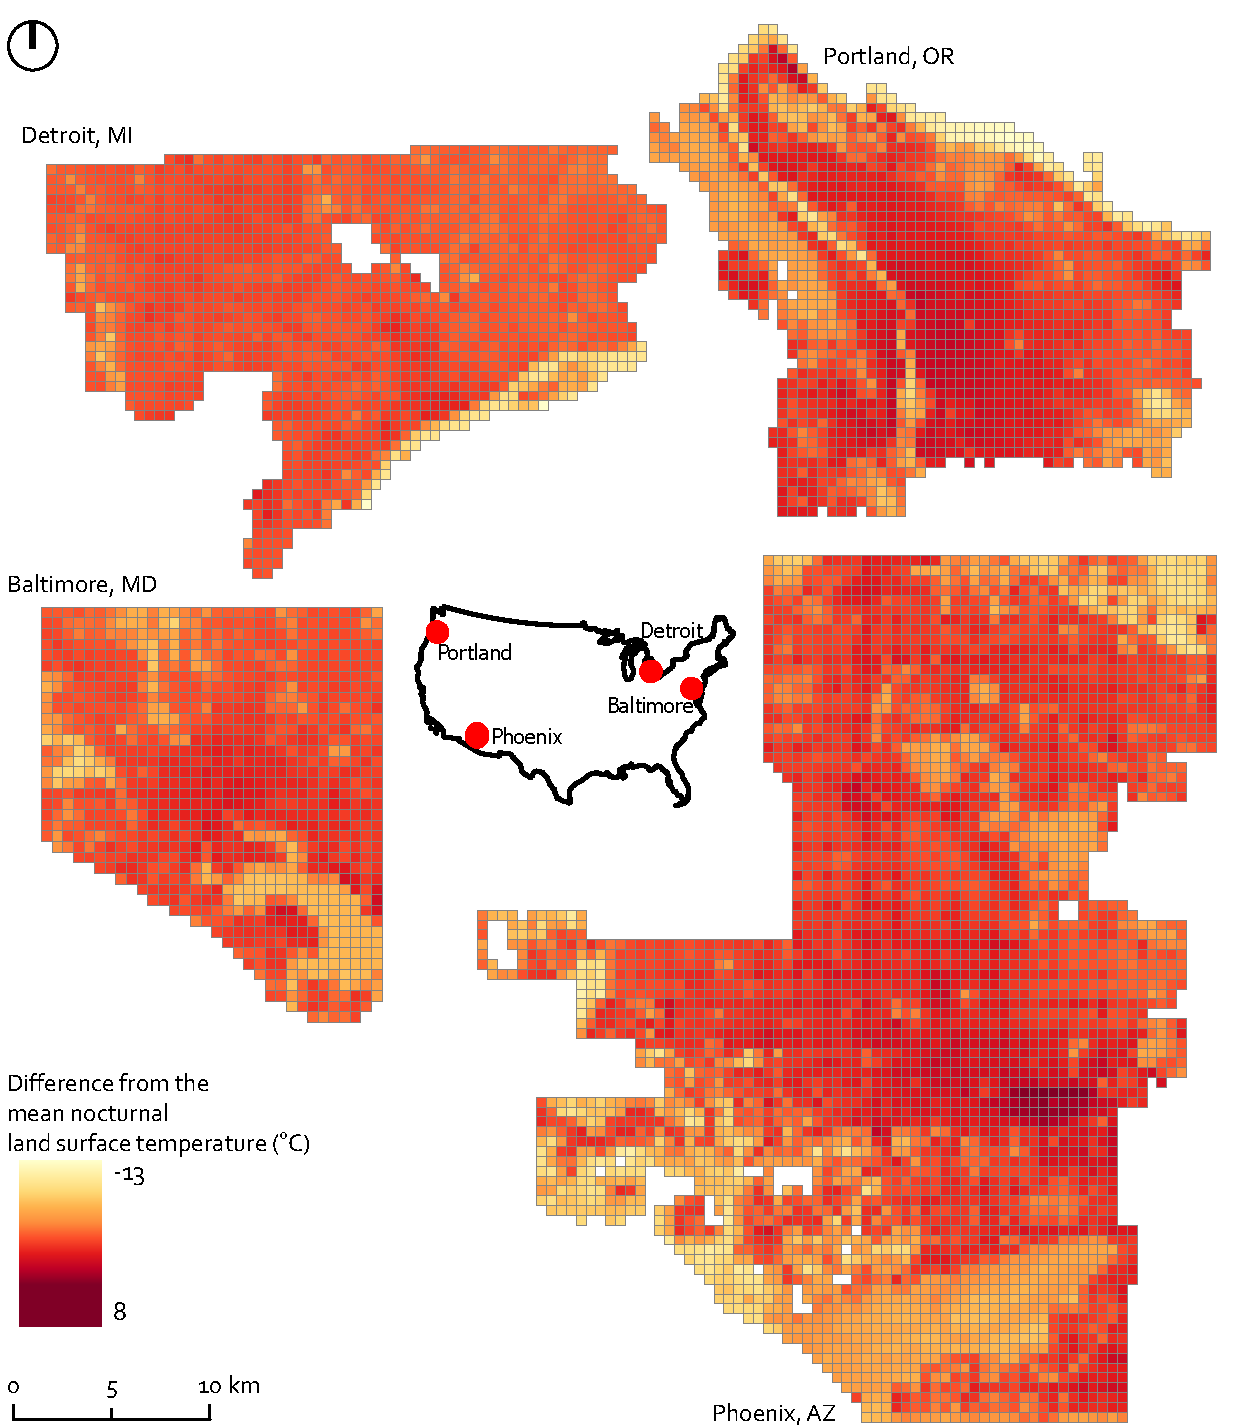
\includegraphics[width=\textwidth]{fig/report/map_nocturnal_lst.pdf}
    \caption{The gridded nocturnal land surface temperature in $^o$C of the cities studied. This is change from the mean (average) for each city.}
    \label{fig:map}
\end{figure*}


\begin{figure}
    \centering
    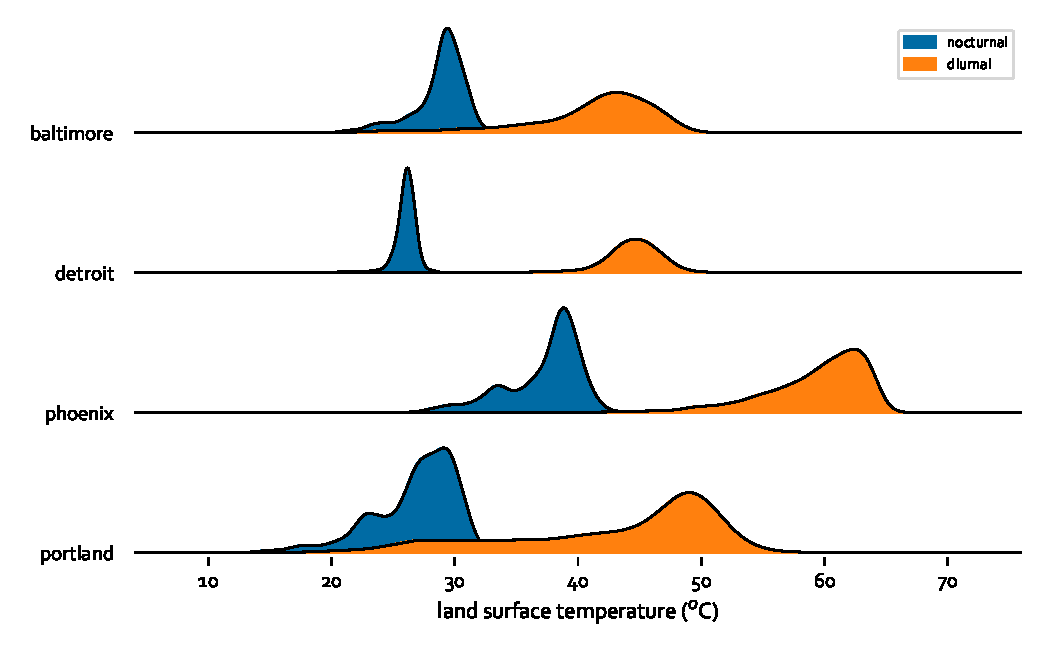
\includegraphics[width=\linewidth]{fig/report/joyplot_lst_500.pdf}
    \caption{The distribution of nocturnal and diurnal land surface temperature of the cities studied.}
    \label{fig:joy}
\end{figure}

\subsection{Land surface temperature}
We calculate land surface temperature using Landsat 8 (Land Processes Distributed Active Archive Center product) imagery as well as land cover and an air temperature observation (data sources provided in \ref{tab:data}. Band-10 digital-number data is converted to top-of-atmosphere radiance \cite{Jimenez-Munoz2003-wc}. We correct for emissivity using land cover data \cite{Alipour2003-gb}, and then calculate the at-satellite brightness temperature \cite{Jimenez-Munoz2003-wc}. Finally an atmospheric correction is made as per the monowindow algorithm \cite{Qin2001-jn} using the maximum observed temperature of the day from a nearby weather station. This follows the process is described in \cite{Scott2016-lc} and is explicit in our open source code on Github\footnote{URL redacted for review}. 

To ameliorate the effect of shadows and other ephemeral changes \cite{Zhou2018-iy} we use at least three minimal-cloud images for each city and night/day period and calculate the mean of LST.

So we can conduct the comparative study between the cities, the land surface temperature for each city is calculated as the difference from the city's mean. 

\begin{figure}
\begin{center}
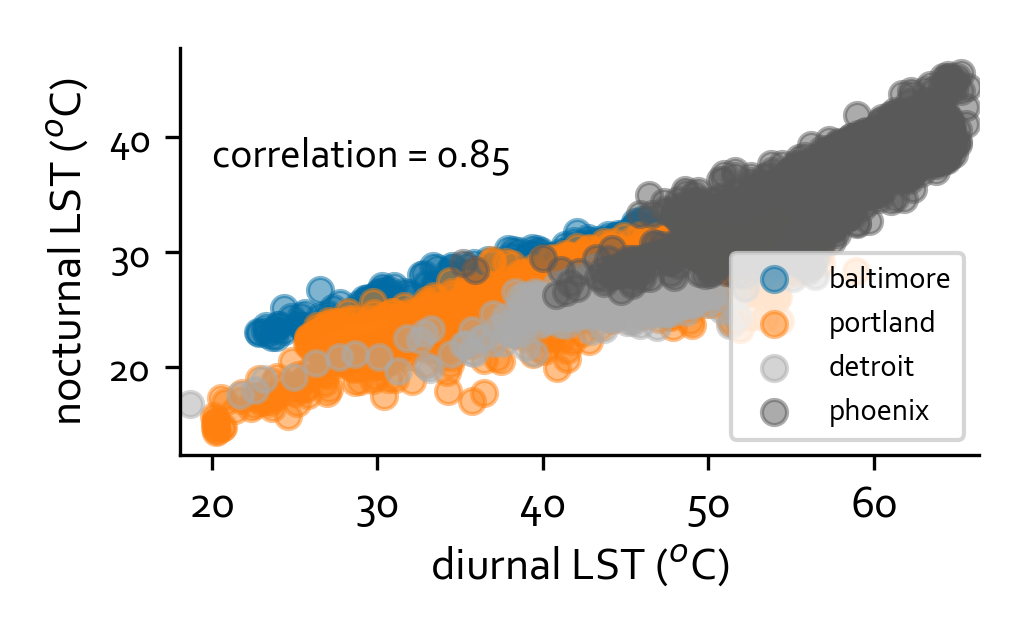
\includegraphics[width=\linewidth]{fig/report/lst_night-vs-day_500.png}
\caption{The land surface temperature in $^o$C of the cities studied at a 500m square resolution}
\label{fig:scatter_lst}
\end{center}
\end{figure}
\subsection{Independent variables}

\textit{Albedo}. Albedo is a measure of the reflectivity or brightness of a surface. It is normalized between 0-1 where the darker surfaces are lower values. Albedo is calculated using the LandSat8 images using the algorithm described in \cite{Smith2010-nw, Liang2001-jd}. 

\textit{Building floor area}. The building floor area within the cell. This uses data released in 2018 by Microsoft where building footprints are estimated using areal images. 

\textit{Building height}. Building height is estimated using the building footprints and available lidar data following \cite{Chun2017-mm}. The mean lidar elevation within each building's footprint is subtracted by the mean digital elevation (topography) within the footprint to estimate the building's height.

\textit{Elevation}. 1/3 arc-second (~10m) bare-earth elevation (topography) data is available courtesy the U.S. Geological Survey. The mean, max, and min of elevation points within the grid cell is calculated.

\textit{Surface elevation}. The surface elevation is determined from the lidar data. Surface elevation captures the natural and built features. 

\textit{Impervious surface percentage}. This is provided in the National Land Cover Database from the Multi-Resolution Land Charasteristic Consortium \cite{Xian2011-aa}. To generate the impervious surface area (ISA) LandSat data, NLCD land cover, and nighttime light imagery is used. The stable nighttime light intensity is only used to estimate the boundary of of urban areas. The Landsat images were converted to top-of-atmosphere reflectance. The data is provided at a 30m resolution and we calculate the mean, max, and min for each grid cell.

**** show scatter against tree canopy - cannot include both ****

\textit{Land cover}. Classification of land cover is described in \cite{Homer2015-ce}. However, as it is used in the calculation of emissivity when calculating the LST it cannot be used as an independent variable. The only landcover that we use is category 11, water. Cells with more than 20\% area classified as water are excluded from the data set.

\textit{NBDI}. Normalized difference built-up index indicates the intensity of imperviousness \cite{Bhatti2014-ae}. It is calculated from satellite images as $$NDVI=\frac{B_{SWIR}-B_{NIR}}{B_{SWIR}+B_{NIR}}$$ where $B_{NIR}$ and $B_{SWIR}$ are the reflectances in the near-infrared and short-wave infrared bands respectively \cite{Alhawiti2016-wv}. Using LandSat8 imagery, this is $$NDVI=\frac{B6-B5}{B6+B5}$$ \cite{barsi2014}.
% *Kaplan 2018, Peng 2018

\textit{NDVI}. The normalized difference vegetation index (NDVI) measures green vegetation. It is calculated from satellite images as $$NDVI=\frac{B_{NIR}-B_{red}}{B_{NIR}+B_{red}}$$ where $B_{NIR}$ and $B_{red}$ are the reflectances in the near-infrared and red bands respectively \cite{Alhawiti2016-wv}. Using LandSat8 imagery, this is $$NDVI=\frac{B5-B4}{B5+B4}$$ \cite{barsi2014}.

% \textit{Nighttime light intensity}. Stable nighttime light intensity is available from the Defense Meteorological Satellite Program (DMSP) Operational Linescan System (OLS). They prepare the data to remove clouds and ephemeral light sources. We use 2013 (the most recently available) data of version 4 at a spatial resolution of 30 arc-seconds (1km at the equator) \cite{ngdc2013version}. The nighttime light intensity was found to be only in moderate agreement with density \cite{bagan2018}, meaning lights may indicate anthropogenic energy use during the night. However, it's lower resolution means that can not capture minor differences. We resampled the raster to a 30m resolution, as per the NLDC \cite{Homer2015-ce}, and for each grid calculated the mean, min, and max.

\textit{Population density}. Density allegedly increases the LST \cite{Li2017-yl}, although this result may be the result of confounding with other factors. Population density calculated from the U.S. census at the block level. The most recent census was 2010, so that data is used as an estimator of where people reside in the evening. This data is also at a lower resolution that the grid cells used, so the grid cell assumes the density of the block that it's centroid is contained within.

\textit{Sky view factor}. Urban canyons have been found to have an effect on UHI because they prevent air circulation \cite{Landsberg1981-mq, Chun2017-mm} and are used to indicate radiation flux within complex environments \cite{Matzarakis2007-xy}. We calculate SVF following using xxx and following the parameters used by \cite{Chun2017-mm}: the number of search directions, $\phi=10^o$; and the radius of the reference circle, $R=300m$. We use a spatial resolution of x-m.
% * Yuan 2011, Unger 2004.

\textit{Tree canopy cover}. The percent tree canopy cover is calculated using National Agriculture Imagery Program (NAIP) aerial imagery, Landsat 5 imagery, elevation, and existing NLCD data \cite{Coulston2012-uu, Homer2015-ce}. The data provided is at an xx resolution. The six reflective bands from Landsat 5 are used to calculate top-of-atmosphere reflectance \cite{Coulston2012-uu} so the data does not contain information used in the LST calculation (which requires radiance). 
% * Rogan 2013, Elmes 2017

\subsection{Data preparation and robustness}

To analyze the data, it needs to transformed into a spatially consistent set.
The raw data is a variety of spatial data types from area level (the population density data), to geostatistical raster (e.g. the land surface temperature).
We choose to resample the data into a grid of square cells.
We conduct the resampling twice to produce a grid of 500m and 100 meter cells. 
Having two grid resolutions allowed us to ensure our conclusions are robust.
For each of the cells the the mean, maximum, and minimum of all variables were calculated. 
To further account for spatial effects of each variable, the mean of the surrounding cells (including diagonal) was calculated and the resulting spatial lag variable was included as an additional independent variable. 
The result is a data set which with we can train a variety of statistical models.

Various statistical models (\S \ref{ss:models}) were trained and then, crucially, validated on unseen data using a technique known as holdout cross-validation. 
This approach partitions 80\% of the data into a training set and the remaining 20\% into the testing set.
The model resulting from the training, is then tested on this unseen test set, to get an estimate of the model accuracy.
This is repeated 100 times and the distribution of the accuracy metric (here we use the mean absolute error (MAE) and variance explained (R$^2$)).
Holdout cross-validation of this type is crucial for statistical analysis to ensure that models are not overfit to data \cite{Geron2017-ek}.
Overfitting occurs when a model fits to the randomness in a dataset, causing it to not be suitable for generalizations. 
When models' accuracy metrics are reported based on in-sample data (the same data it was trained on), the accuracy metrics are high.
This is essential for statistical models and overlooked by the majority of existing studies (e.g. \cite{Zhou2014-wc, Peng2018-cp, Chun2017-mm, Chun2018-so,Wang2019-tree}).
Cross-validation helps to avoid this by evaluating the model on unseen data.

A further way to avoid overfitting is to carefully consider how the test data is selected.
This is especially important with spatial data.
Therefore, when selecting the test and training data the grid cells were grouped into a larger 8x8 grid.
This avoids over fitting of the model by training the model on a cell adjacent to a cell that is included in the test set.

Finally, we attempt to capture uncertainty in the data and the models. 
To represent the data uncertainty we conduct randomly sample from our data to create a new dataset.
The models are trained on this new dataset and this is repeated.
This approach, known as bootstrapping, means that the conclusions' sensitivity to the data can be assessed.
If the results are vastly different for each bootstrap sample, we assume that the result is dependent on the data and is unlikely to be generalizable to other cities.
Additionally, we capture model uncertainty by using different models and assessing how each model shows the urban characteristics influencing the land surface temperature.
If all bootstrapped models are generally in agreement, it suggests that the conclusions are robust.

\subsection{Statistical models}
\label{ss:models}
The relationship between urban characteristics and land surface temperature is complex.
This complexity may not be captured by a linear regression model. 
We fit a series of regression and data-mining models to the data and their predictive accuracy and variable association are compared.

\textit{Null model: average}. The first model, to compare other models against, is the null model. 
This is a benchmark model to ensure the models we fit are not doing worse than no model.
The mean, average, of the observations is calculated and is used as the prediction for the test observations.

\textit{Linear model}. Linear models are suitable when there is a linear relationship between the explanatory variables (urban characteristics) and the response variable (LST).

\textit{Multivariate Adaptive Regression Spline (MARS)}. The MARS model extends the linear model, by using piece-wise functions to fit the data. \cite{Friedman1991-of}

\textit{Generalized Additive Model (GAM)}. The GAM is also an extension of the linear model, although it does not require a linear relationship. Instead, the response variable is estimated as the sum of smoothing functions that are applied to each covariate \cite{Hastie1990-cg}.

\textit{Random Forest}. A random forest is an ensemble model of \textit{Regression Trees}. A regression tree partitions the data based on thresholds for the covariates \cite{Breiman1984-hw}. It continues to divide the data on different covariates until the partitions are as similar as possible. 
The result is a tree-like structure, after which the model is named.
In similar naming fashion, a random forest is a collection of regression trees.
Each tree is \textit{grown} from a random subset of the data and the prediction from the random forest model is the average of the prediction from all of the trees \cite{Breiman2001-rt}.

\textit{Gradient Boosted Regression Trees}. This is similar to the random forest, that it is a collective of regression trees. 
However, the difference is that each tree is trained sequentially on the residuals of the previous tree.
The result is the average of all of the regression trees \cite{Geron2017-ek}.

\section{Results and Discussion}

During the day, Increased impervious surfaces and decreased vegetation increase sensible heat flux and lower latent heat flux \cite{Voogt2003-mm, Peng2012-iy, Zhou2014-wc}

Heat storage during the day, increases temperatures during the night \cite{Voogt2003-mm, Zhou2014-wc}

Day and night mechanisms that drive temperature differ, likely because latent and sensible heat dominant during the day, but ground heat flux dominates at night \cite{Zhou2014-wc, Voogt2003-mm}.

Vegetation and pervious surfaces caused the greatest reduction in land surface temperature, with approximately 10oC change during the day (Figure \ref{fig:pdp_2dday_500}b). 
This result supports existing findings \cite{Zhou2014-wc, Chun2018-so}.
it is likely due to vegetation increasing the latent heat fluxes due to transpiration \cite{Zhou2014-wc}, which explains why it has a greater effect during the day. 
vegetation does not transpire during the night however, so the reduction in temperature due to increased tree cnaopy cover, is likely due to a reduction in impervious surfaces that store heat \cite{Voogt2003-mm}. 
Not all types of pervious surfaces are as good as others \cite{Gober2009-im}. Care must be taken when irrigating \cite{Gober2009-im}.
urban design needs to consider interaction between surface materials \cite{Guhathakurta2010-ib}.
- vegetation important during the day \cite{Chun2017-mm, Peng2018-cp}
- vegetation is important \cite{Wang2019-tree}

water
- showed no effect in the 100m data, because so few data observations had water in them.
- dramatic reductions in temperature during both night and day (y $^o$C).
- this contrasts with findings and rationale that water releases heat at night \cite{Chun2017-mm} - although that logic applies to air temperature, not sure how strong water would be at increasing temperature of nearby land surface
- supports strong negative findings \cite{Wang2019-water}

Urbanization leads to heat storage in roads and buildings \cite{Zhou2014-wc, Voogt2003-mm}. 
the results were surpringly inconsistent, regarding albedo - however, this is confounded as vegetation and highly impervious surfaces are both dark (low albedo).
considering 2d partial dependence, we see that albedo has little affect at night it does show that the highest temperatures are the most built up and the least reflective (Figure \ref{fig:pdp_2dnight_500}a).
during the day, tincreasing the whiteness, decreases the temperature. the higest temperatures are observed when there is significant building area and low albedo (Figure \ref{fig:pdp_2dday_500}a) and high impervious area and low albedo (Figure \ref{fig:pdp_2dday_500}b).
- albedo, then ndbi to be most important, only consider day \cite{Peng2018-cp}
- role of impervious surface \cite{Lu2006-ch}



The canyon effect is also attributed to cause warmer temperatures. \cite{Chun2017-mm,Oke1988-re}
while there was high uncertainty in the models, it appears that during the night, the temperatures decrease as the sky view factor increased (Figure \ref{fig:pdp_night_500}d).
This is potentially due to heat being stored within the canyons (areas with low, sky view factors).
Conversely, during the day, areas with high sky view factor had increased temperature (Figure \ref{fig:pdp_day_500}d).
This is may be a result of shade from the buildings \cite{Yu2019-ps}.
Urban canyon was found to be important at night \cite{Chun2017-mm}



The building area had no affect during the night (Figure \ref{fig:pdp_night_500}) and increased temperature during the day (Figure \ref{fig:pdp_day_500}).
The population density had no discernible affect during night or day.



Supports suggestion that 2D metrics outperform 3D metrics \cite{Berger2017-lx}


\begin{figure*}
    \centering
    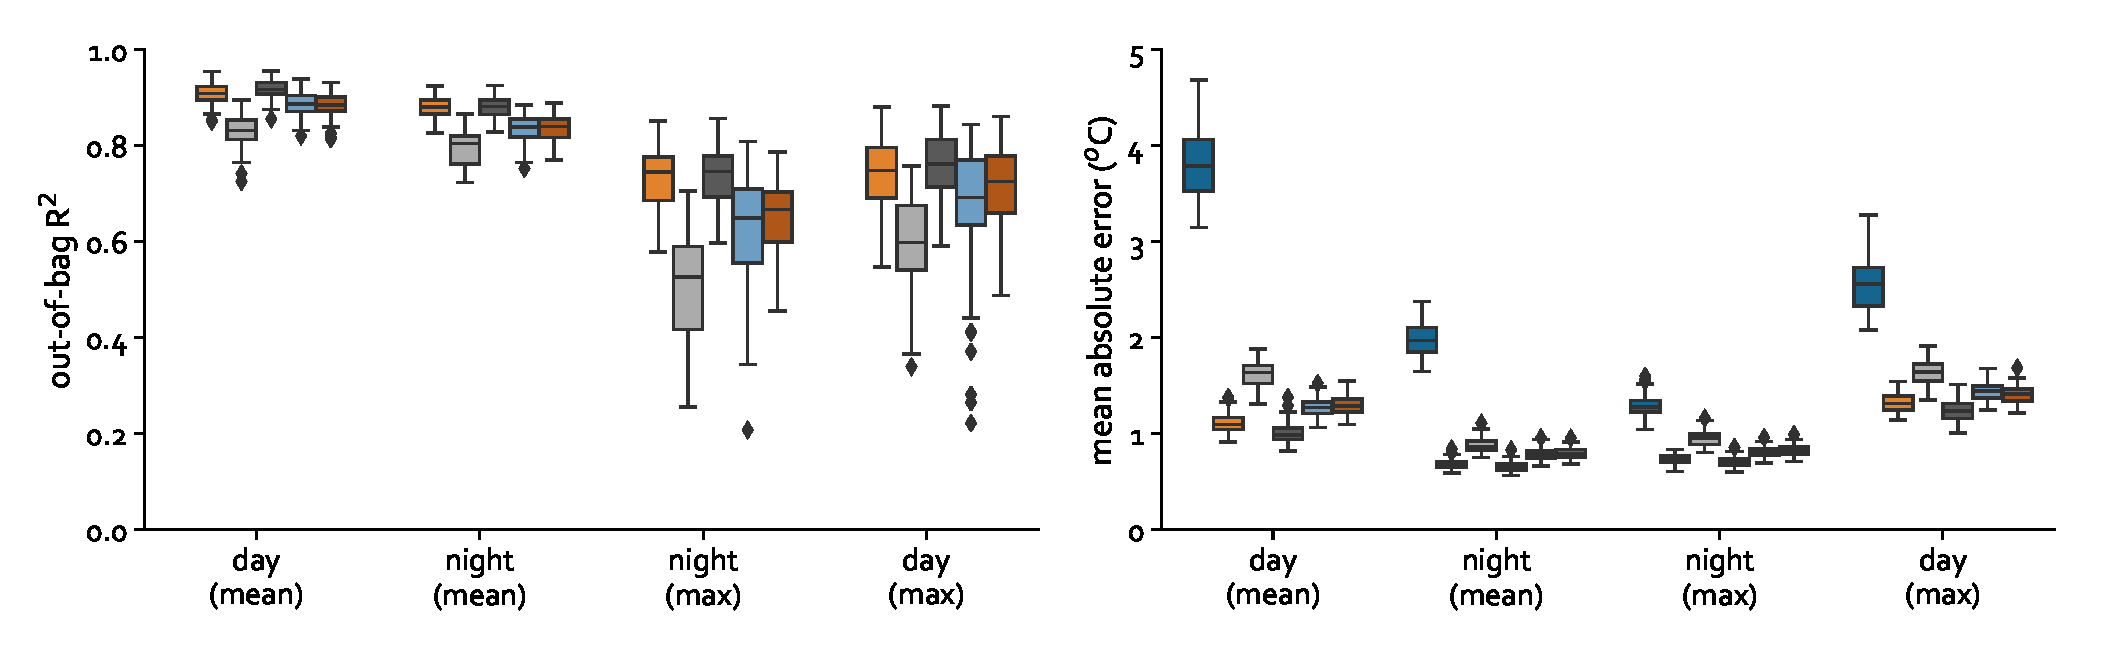
\includegraphics[width=\linewidth]{fig/report/holdout_results_500.pdf}
    \caption{
    The out-of-bag (OOB) R$^2$ and mean absolute error (MAE) of the models when fitted on three of the four cities and then used to predict the remaining city. OOB R$^2$ can vary between $(-\infty, 1)$, where better models have a value near 1. Good models have MAE near 0. The gradient boosted regression forest generally outperforms the other models, except when predicting Detroit. Note that the R$^2$ axis is truncated at -1, although the multiple linear regression for diurnal land surface temperature tested on Phoenix has an OOB R$^2$ of -9.  This shows that the gradient boosted regression forest (gbm) consistently outperforms the multiple linear regression and null models.
    }
    \label{fig:holdout_500}
\end{figure*}

\begin{figure*}
\begin{center}
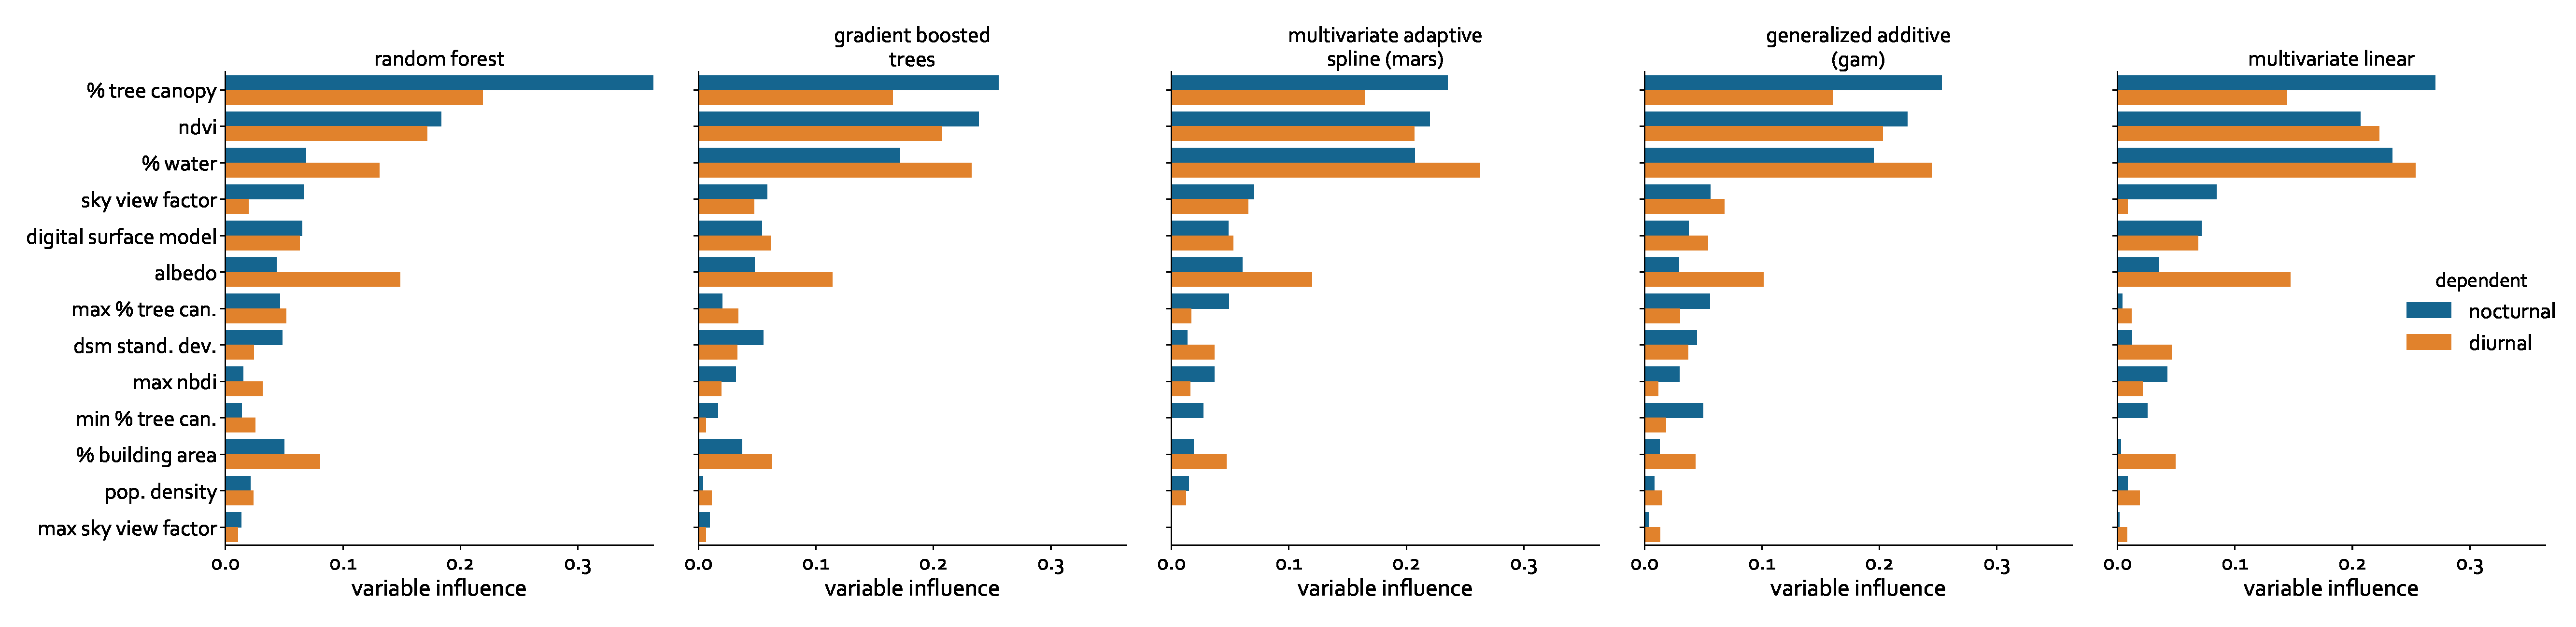
\includegraphics[width=\textwidth]{fig/report/variableImportance_500.pdf}
\caption{The variable importance for the regression during the night (to the left) and the day (to the right). Variable importance indicates the amount that each variable improves the performance of the regression.
In this case there is generally little difference between the importance of day and night variables.}
\label{fig:importance_500}
\end{center}
\end{figure*}


\begin{figure*}
    \centering
    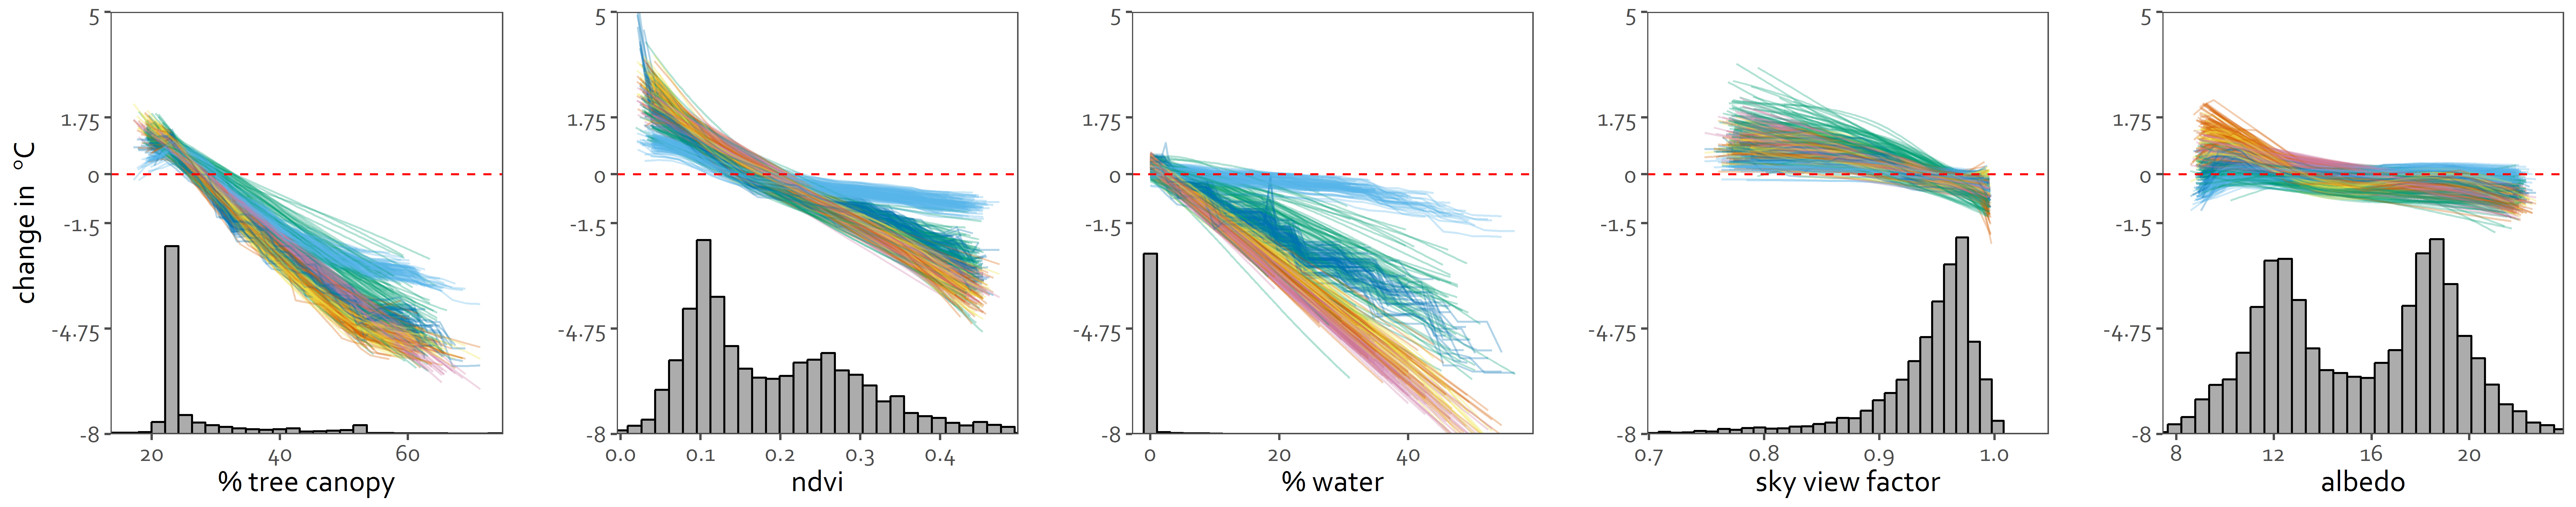
\includegraphics[width=\linewidth]{fig/report/pdp_uncert_night_500.png}
    \caption{
    Partial dependence plots show how the land surface temperature ($^oC$, y axis) changes with each variable as the other variables are held at their average value. The left hand side shows the effect each variable has on LST during the night, while the right hand side shows the effect during the day. This shows that trees coverage in the cell has the greatest influence on the temperature, and the greenness (NDVI) of that coverage matters during the day.
    }
    \label{fig:pdp_night_500}
\end{figure*}

\begin{figure*}
    \centering
    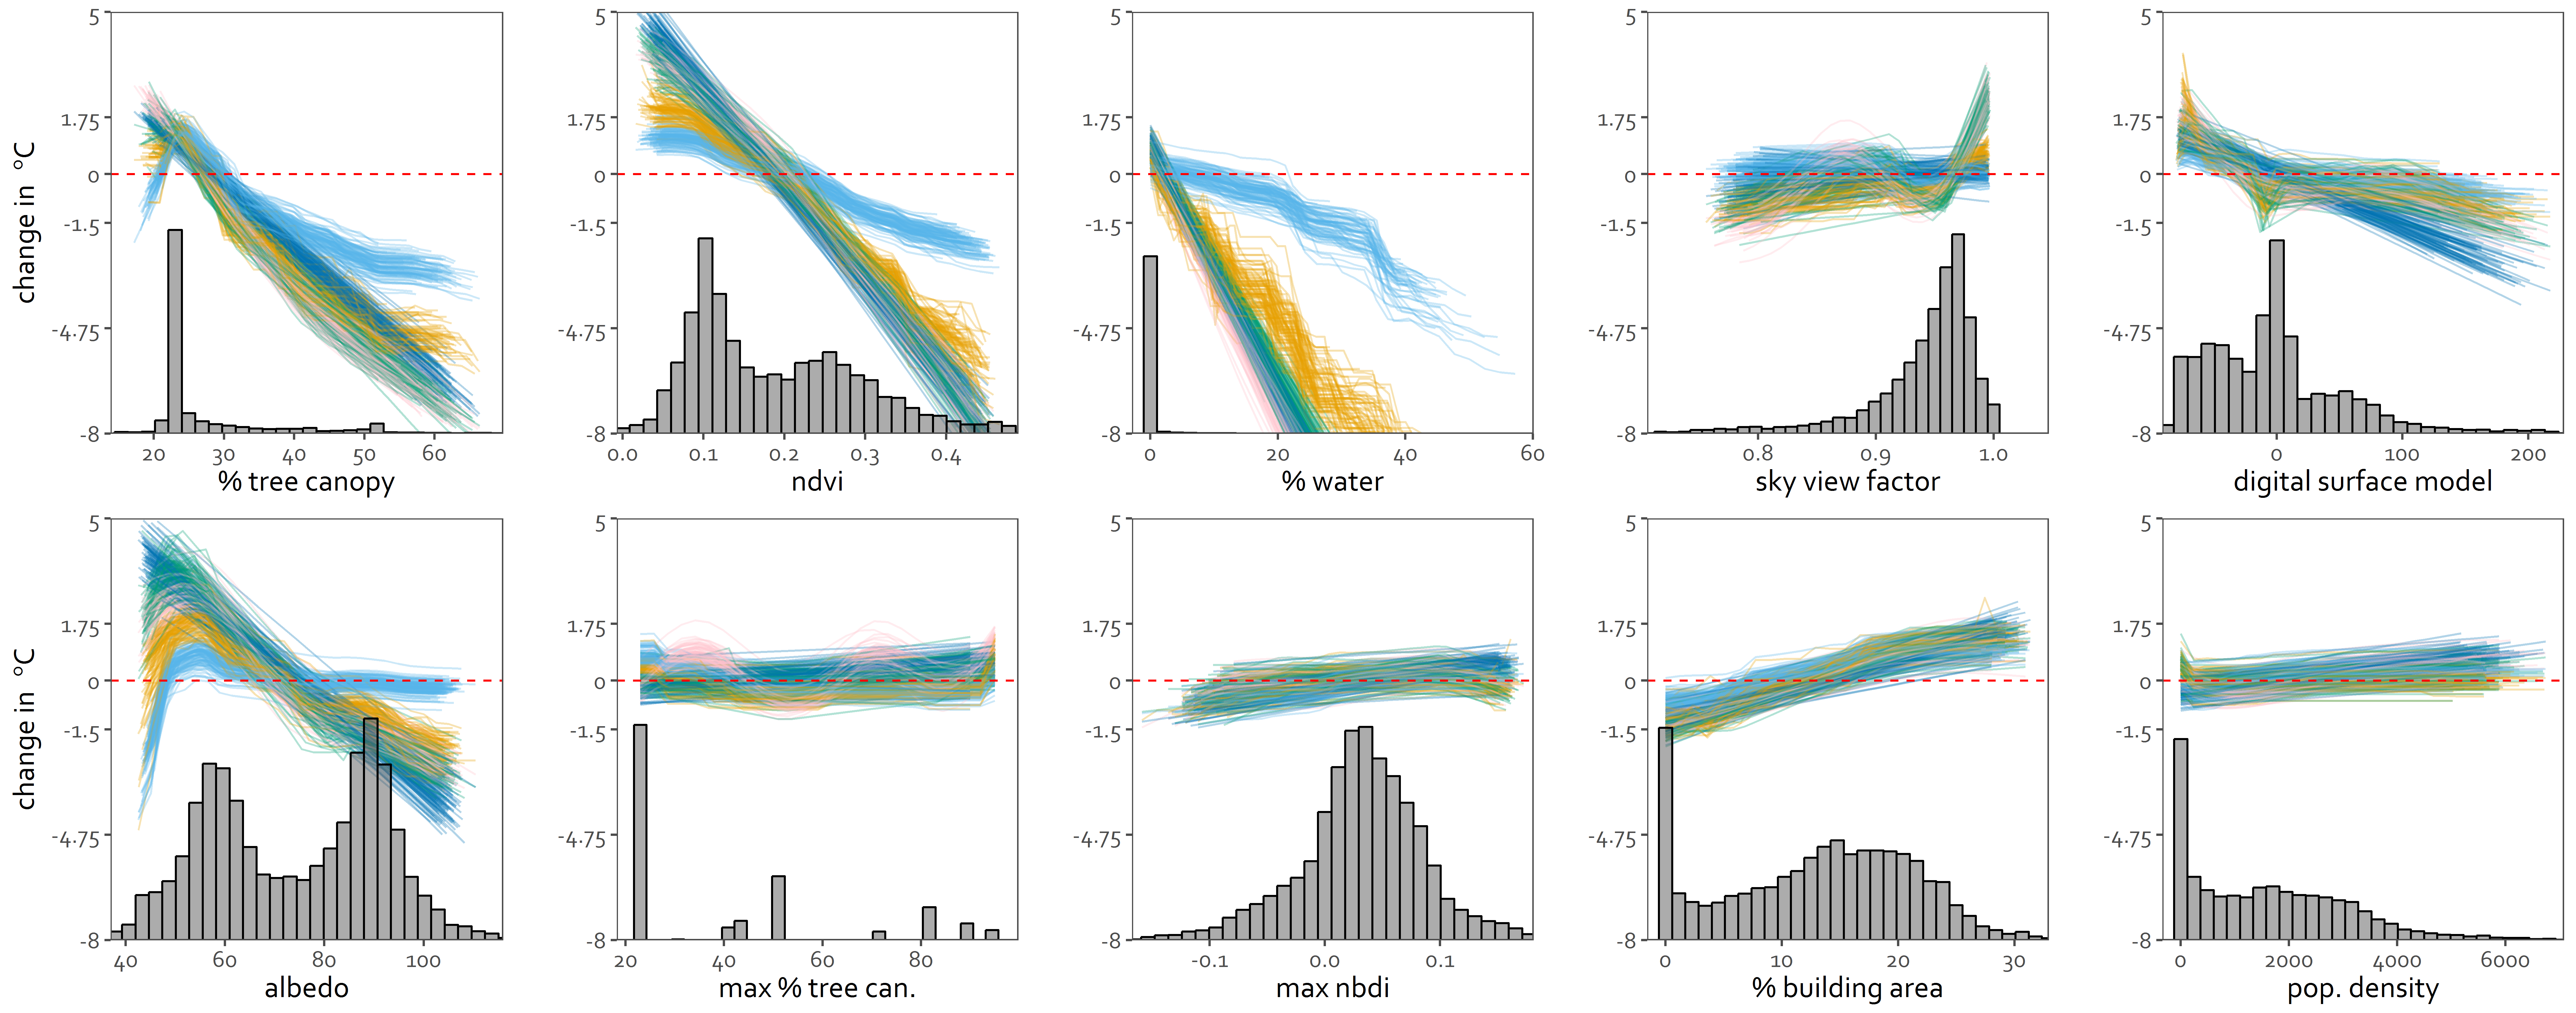
\includegraphics[width=\linewidth]{fig/report/pdp_uncert_day_500.png}
    \caption{
    Partial dependence plots show how the land surface temperature ($^oC$, y axis) changes with each variable as the other variables are held at their average value. The left hand side shows the effect each variable has on LST during the night, while the right hand side shows the effect during the day. This shows that trees coverage in the cell has the greatest influence on the temperature, and the greenness (NDVI) of that coverage matters during the day.
    }
    \label{fig:pdp_day_500}
\end{figure*}

\begin{figure*}
    \centering
    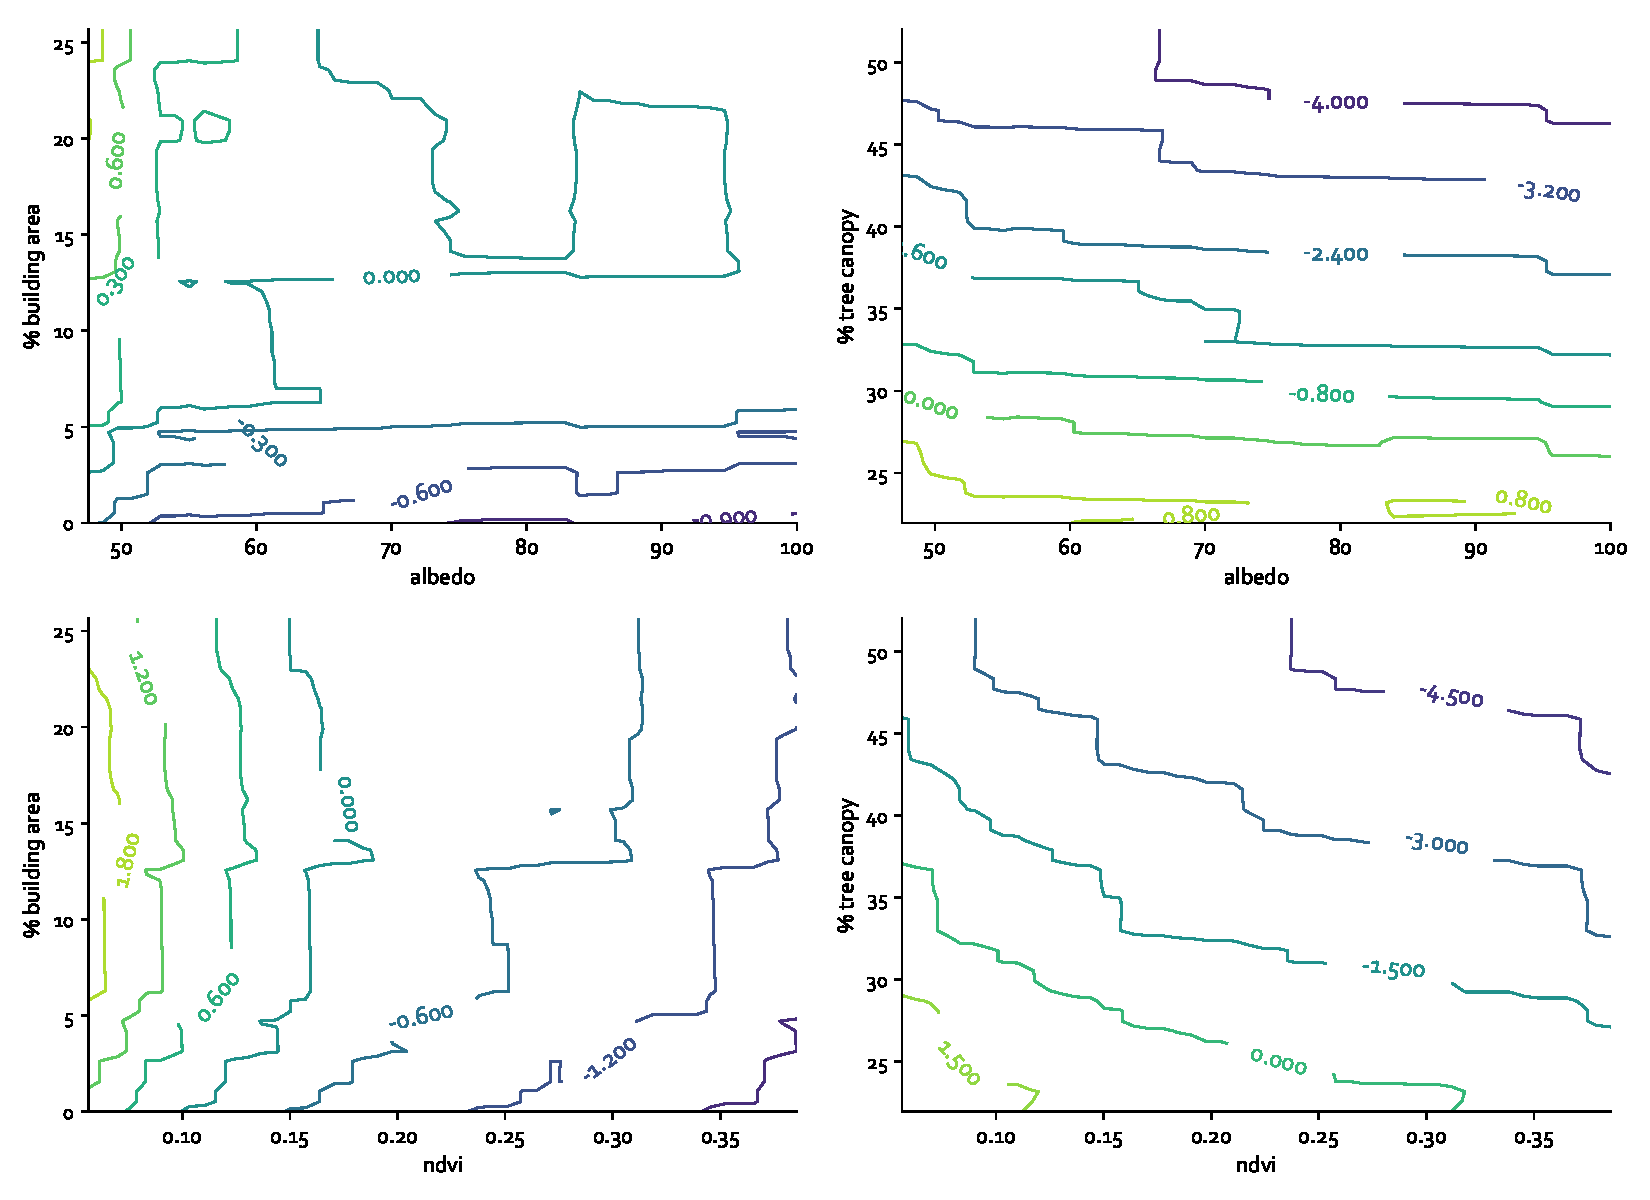
\includegraphics[width=\linewidth]{fig/report/pdp_2d_night_500.pdf}
    \caption{
    Partial dependence plots show how the land surface temperature ($^oC$, y axis) changes with each variable as the other variables are held at their average value. The left hand side shows the effect each variable has on LST during the night, while the right hand side shows the effect during the day. This shows that trees coverage in the cell has the greatest influence on the temperature, and the greenness (NDVI) of that coverage matters during the day.
    }
    \label{fig:pdp_2dnight_500}
\end{figure*}

\begin{figure*}
    \centering
    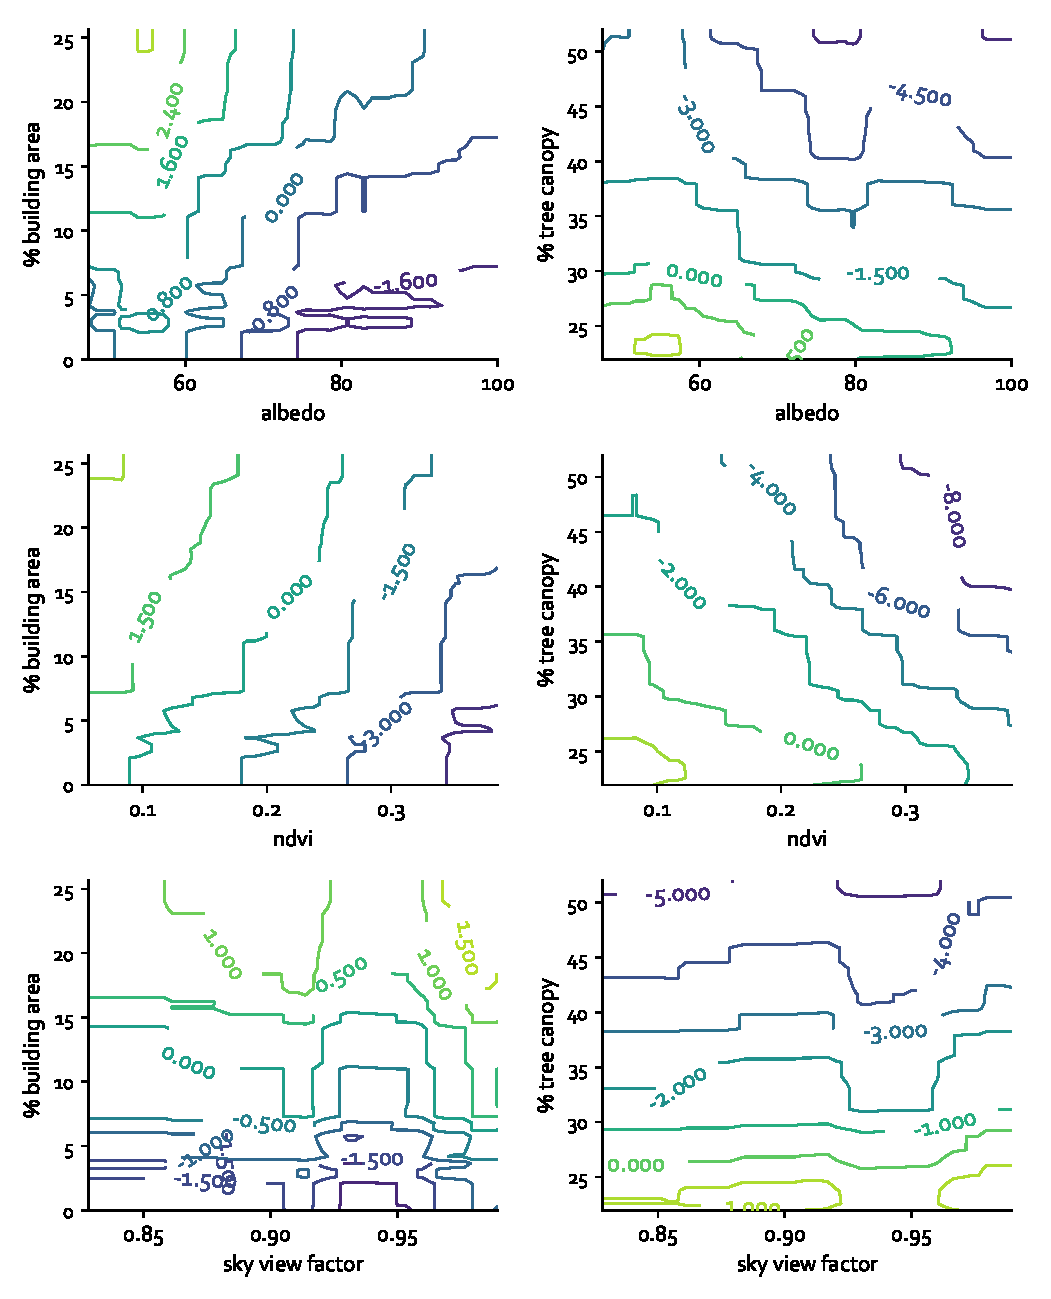
\includegraphics[width=\linewidth]{fig/report/pdp_2d_day_500.pdf}
    \caption{
    Partial dependence plots show how the land surface temperature ($^oC$, y axis) changes with each variable as the other variables are held at their average value. The left hand side shows the effect each variable has on LST during the night, while the right hand side shows the effect during the day. This shows that trees coverage in the cell has the greatest influence on the temperature, and the greenness (NDVI) of that coverage matters during the day.
    }
    \label{fig:pdp_2dday_500}
\end{figure*}






\section{Conclusion}

We analyzed ...

Tree canopy, impervious surface, and greeness had the largest effect on temperature during the night (change of x oC).
During the day xyz

Our results highlight 

This work strongly supports initiatives for increasing green infrastructure in cities \cite{Larsen2015-da, Meerow2017-xv}. 
conducting a thorough nonlinear statistical analysis that accounts for seasonality is the next step to ensuring that interventions are effective year-round.

It does not support claims that constrain floor area ratios, which would lead to reduced density \cite{Chun2017-mm}. 
A further necessary study is to compare sprawling and dense cities, before steps to dissuade density are taken. 
And steps such as vertical and horizontal randomness of buildings or simply green roofs may be what is required \cite{Gago2013-ta}.
highlights the importance of urban planning strategies and studies that can quantify these would be valuable.

To mitigate the effects of future heat waves, cities need to reduce their impervious surfaces and increase the amount of vegetation.

% There are various bibliography styles available. You can select the style of your choice in the preamble of this document. These styles are Elsevier styles based on standard styles like Harvard and Vancouver. Please use Bib\TeX\ to generate your bibliography and include DOIs whenever available.

% Here are two sample references: \cite{Feynman1963118,Dirac1953888}.
\section*{Acknowledgements}
TML - Hazard SEES, Rackham PreDoctoral
What else?


\section*{References}

\bibliography{mybibfile.bib}

\newpage
\onecolumn
\appendix

\section{Data sources}

\begin{tabu}to \textwidth{ X[l]  X[c]  X[c] X[l] X[l] }
 \hline
 Data Provider & Data Type & Data Date & Description & URL \\
 \hline
U.S. Geological Survey  & Raster  & 2013-2017 &
    Landsat 8 day and night satellite imagery & \burl{https://earthexplorer.usgs.gov/} \\
Microsoft  & Polygon  & 2018 & Building footprint polygons for the US &
    \burl{https://github.com/Microsoft/USBuildingFootprints} \\
Defense Meteorological Satellite Program  & Raster  & 2013 &
    Stable nighttime light intensity & \burl{https://www.ngdc.noaa.gov/eog/dmsp/downloadV4composites.html} \\
Multi-Resolution Land Characteristics Consortium  & Raster  & 2011 &
    Land cover & \burl{https://www.mrlc.gov} \\
Multi-Resolution Land Characteristics Consortium  & Raster  & 2011 &
    Percent developed imperviousness & \burl{https://viewer.nationalmap.gov} \\
Multi-Resolution Land Characteristics Consortium  & Raster  & 2011 &
    Percent tree canopy cover & \burl{https://viewer.nationalmap.gov} \\
U.S. Geological Survey  & Raster  & 2015 & 1/3 arc-second elevation &
    \burl{https://nationalmap.gov/3DEP/3dep_prodserv.html} \\
U.S. National Oceanic and Atmospheric Administration  & Lidar  & 2014 & Point cloud of surface elevation &
    \burl{https://coast.noaa.gov/htdata/lidar2_z/geoid12b/data/6377/} \\
IPUMS NHGIS  & Area Level  & 2010 &
    Block-level population from the US census & \cite{nhgis}\\
\hline
\label{tab:data}
\end{tabu}




\section{Additional model results}
\begin{figure}
    \centering
    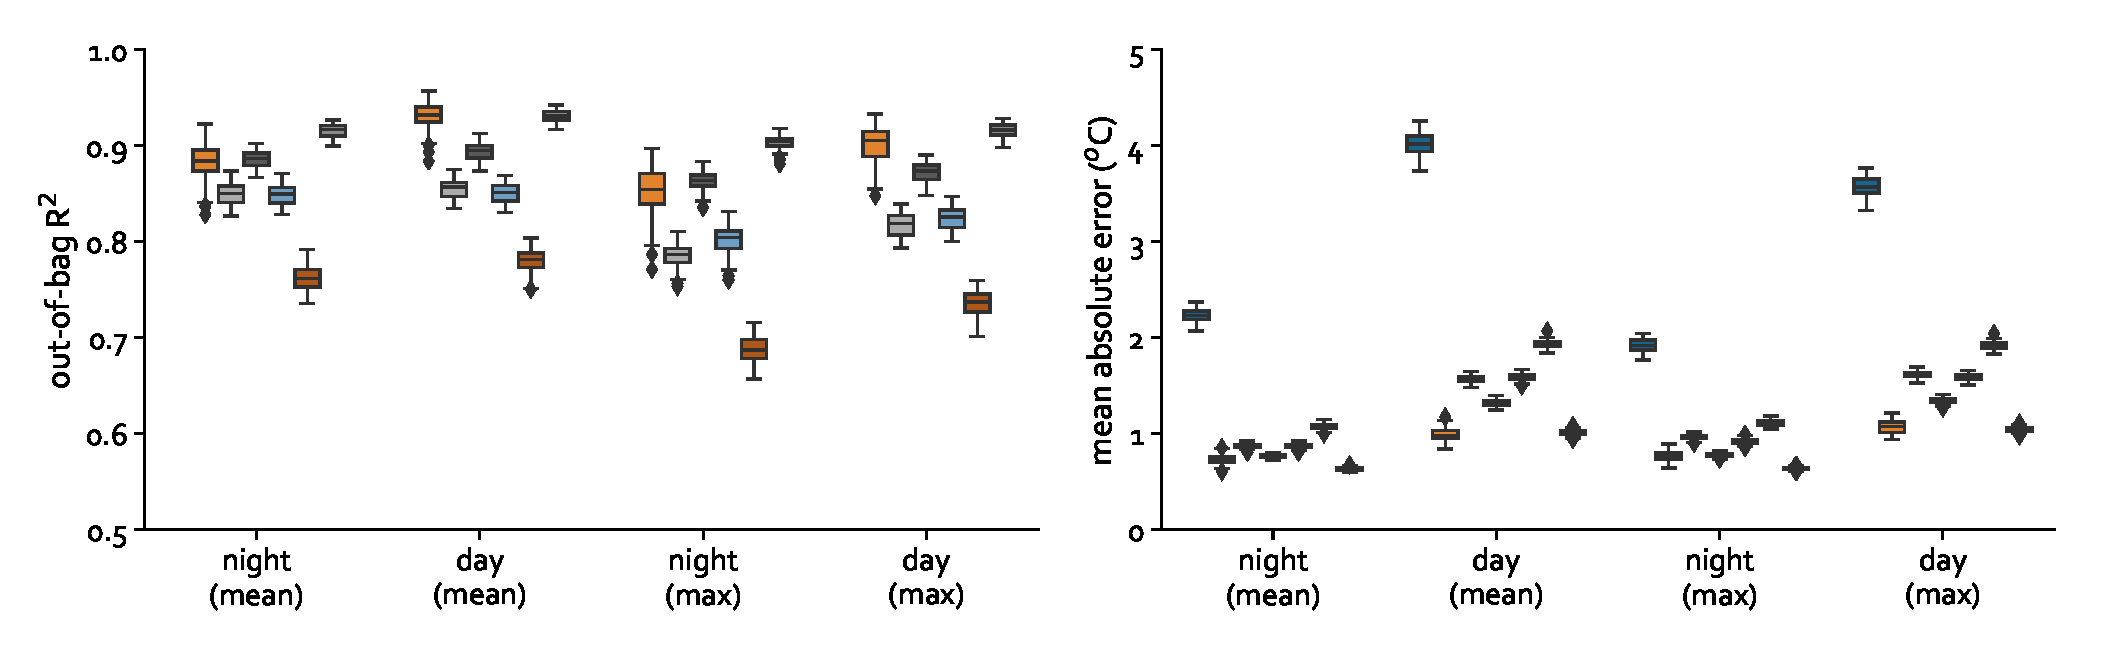
\includegraphics[width=\linewidth]{fig/report/holdout_results_100.pdf}
    \caption{
    The out-of-bag (OOB) R$^2$ and mean absolute error (MAE) of the models when fitted on three of the four cities and then used to predict the remaining city. OOB R$^2$ can vary between $(-\infty, 1)$, where better models have a value near 1. Good models have MAE near 0. The gradient boosted regression forest generally outperforms the other models, except when predicting Detroit. Note that the R$^2$ axis is truncated at -1, although the multiple linear regression for diurnal land surface temperature tested on Phoenix has an OOB R$^2$ of -9.  This shows that the gradient boosted regression forest (gbm) consistently outperforms the multiple linear regression and null models.
    }
    \label{fig:holdout_results}
\end{figure}



\begin{figure}
\begin{center}
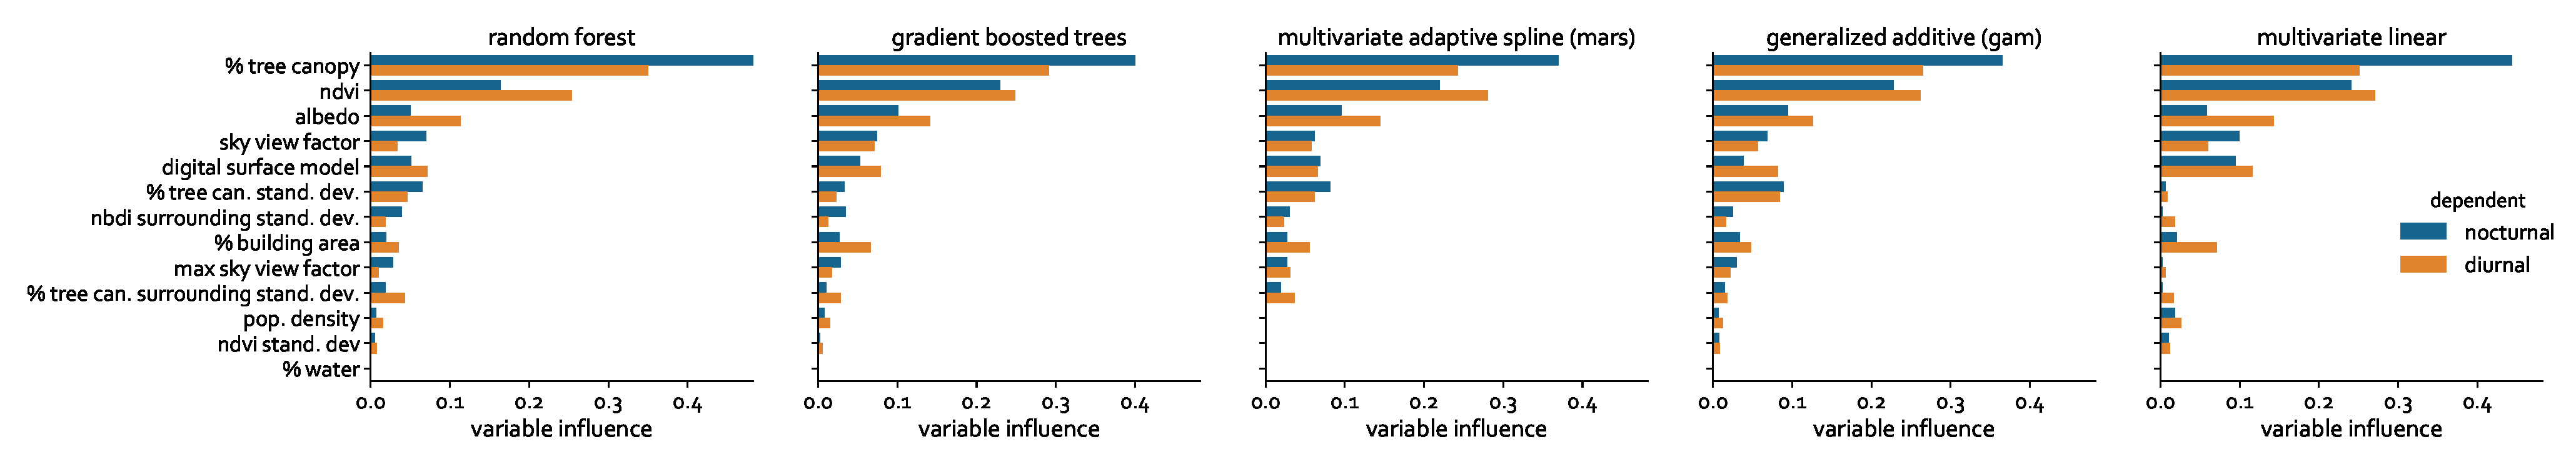
\includegraphics[width=\textwidth]{fig/report/variableImportance_100.pdf}
\caption{The variable importance for the regression during the night (to the left) and the day (to the right). Variable importance indicates the amount that each variable improves the performance of the regression.
In this case there is generally little difference between the importance of day and night variables.}
\label{fig:importance}
\end{center}
\end{figure}


\begin{figure}
    \centering
    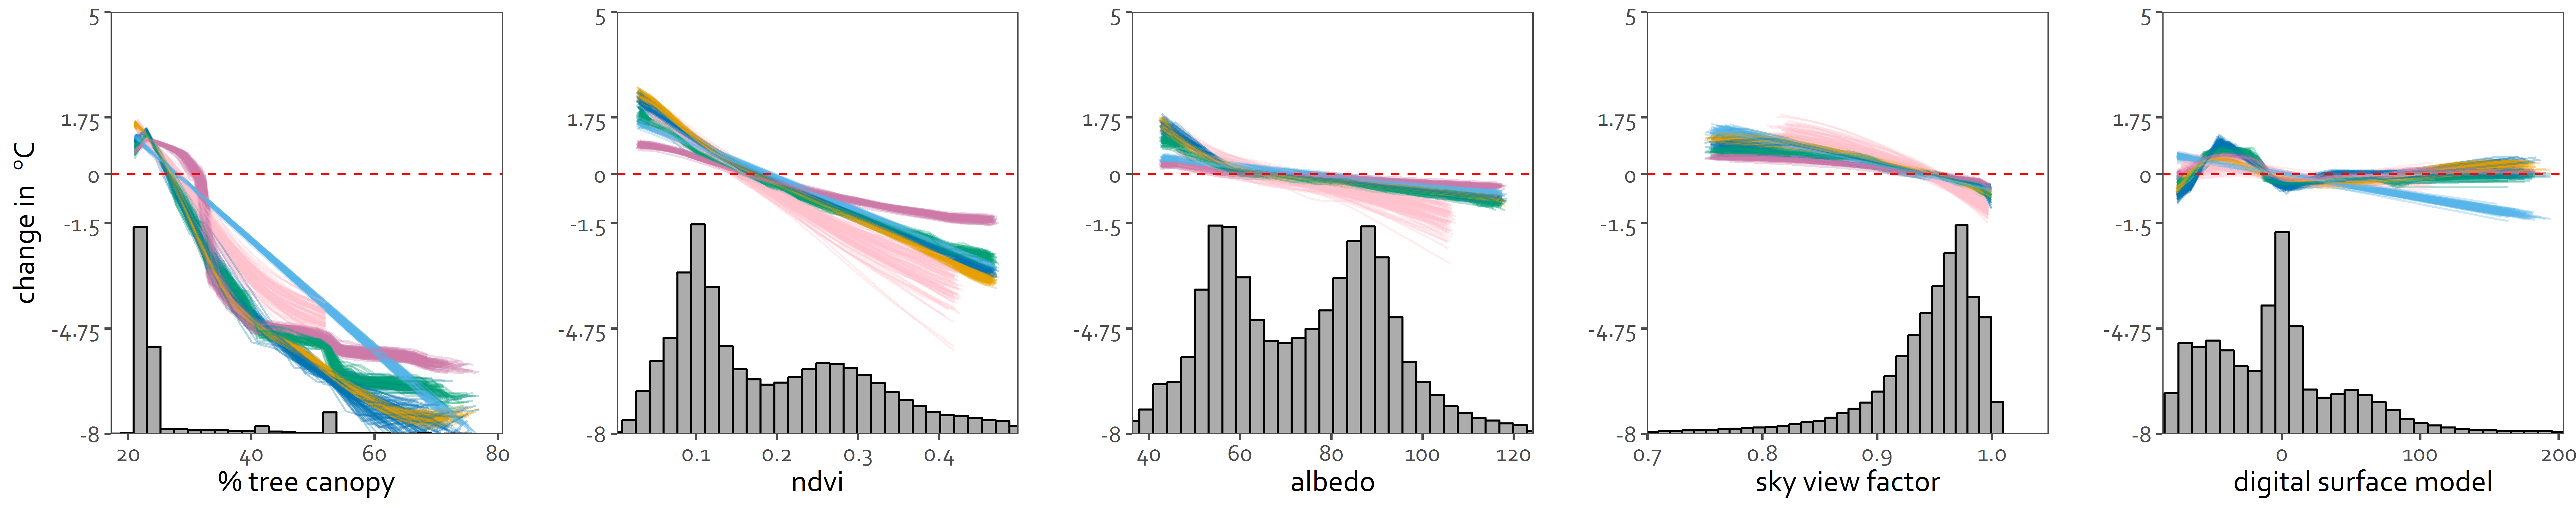
\includegraphics[width=\linewidth]{fig/report/pdp_uncert_night_100.png}
    \caption{
    Partial dependence plots show how the land surface temperature ($^oC$, y axis) changes with each variable as the other variables are held at their average value. The left hand side shows the effect each variable has on LST during the night, while the right hand side shows the effect during the day. This shows that trees coverage in the cell has the greatest influence on the temperature, and the greenness (NDVI) of that coverage matters during the day.
    }
    \label{fig:pdp_night}
\end{figure}

\begin{figure}
    \centering
    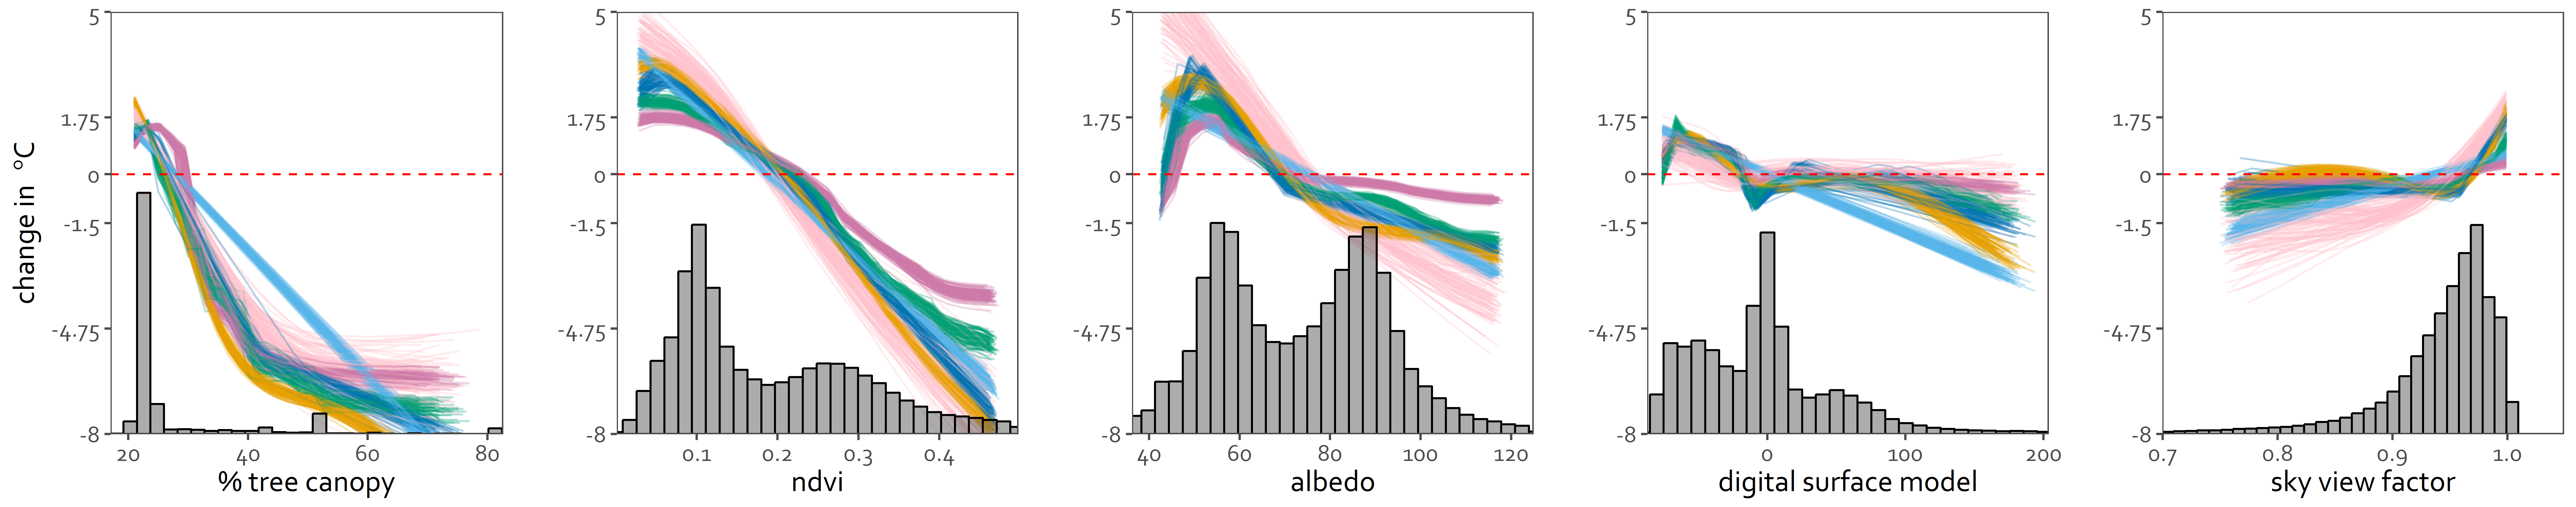
\includegraphics[width=\linewidth]{fig/report/pdp_uncert_day_100.png}
    \caption{
    Partial dependence plots show how the land surface temperature ($^oC$, y axis) changes with each variable as the other variables are held at their average value. The left hand side shows the effect each variable has on LST during the night, while the right hand side shows the effect during the day. This shows that trees coverage in the cell has the greatest influence on the temperature, and the greenness (NDVI) of that coverage matters during the day.
    }
    \label{fig:pdp_day}
\end{figure}

\begin{figure}
    \centering
    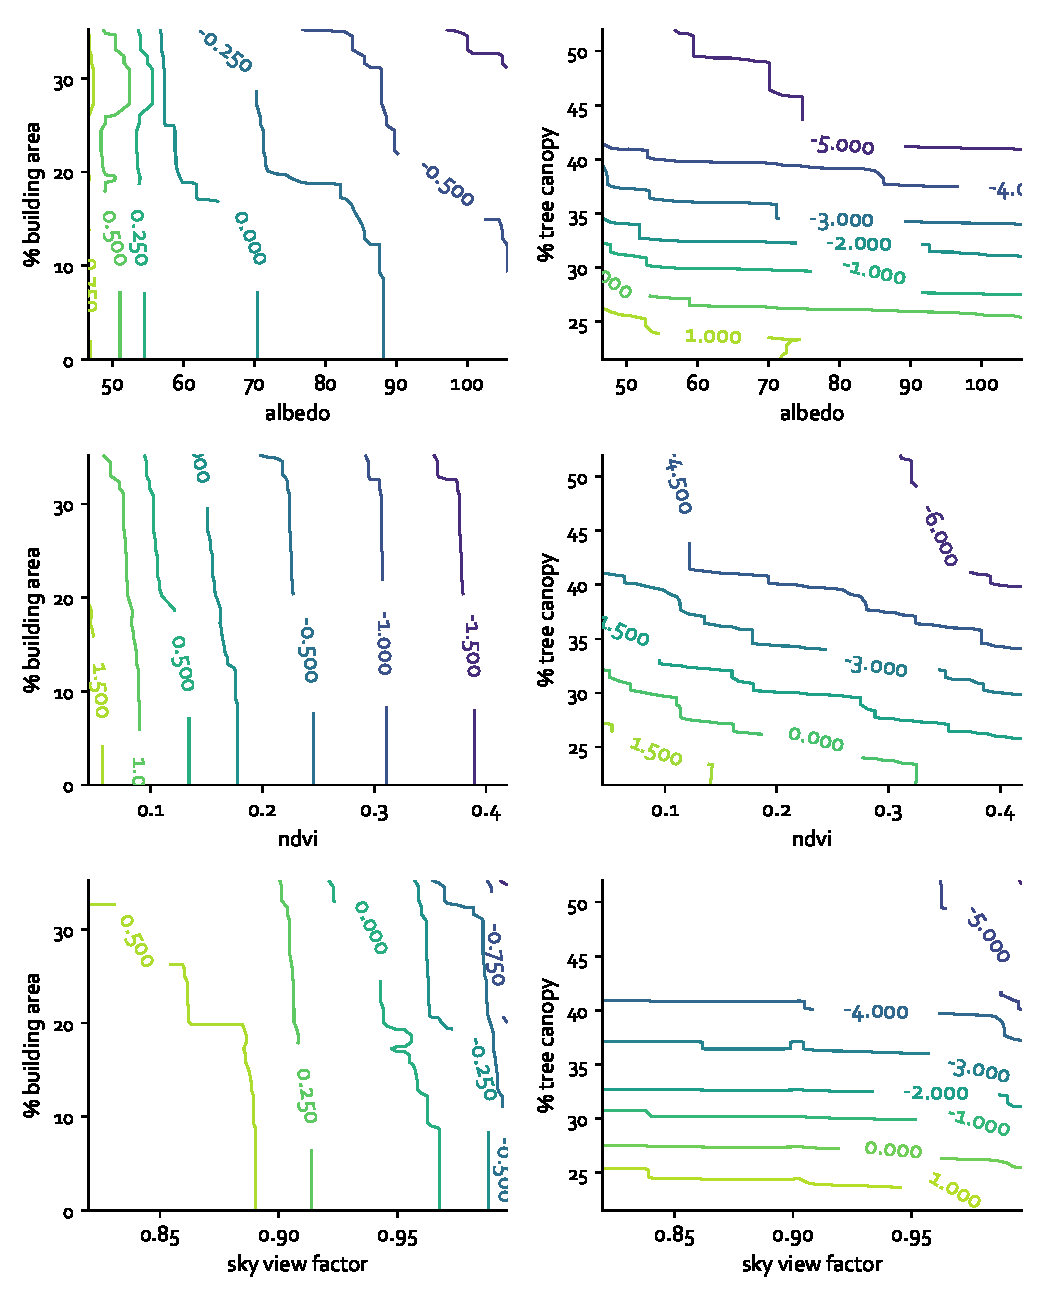
\includegraphics[width=\linewidth]{fig/report/pdp_2d_night_100.pdf}
    \caption{
    Partial dependence plots show how the land surface temperature ($^oC$, y axis) changes with each variable as the other variables are held at their average value. The left hand side shows the effect each variable has on LST during the night, while the right hand side shows the effect during the day. This shows that trees coverage in the cell has the greatest influence on the temperature, and the greenness (NDVI) of that coverage matters during the day.
    }
    \label{fig:pdp_2dnight}
\end{figure}

\begin{figure}
    \centering
    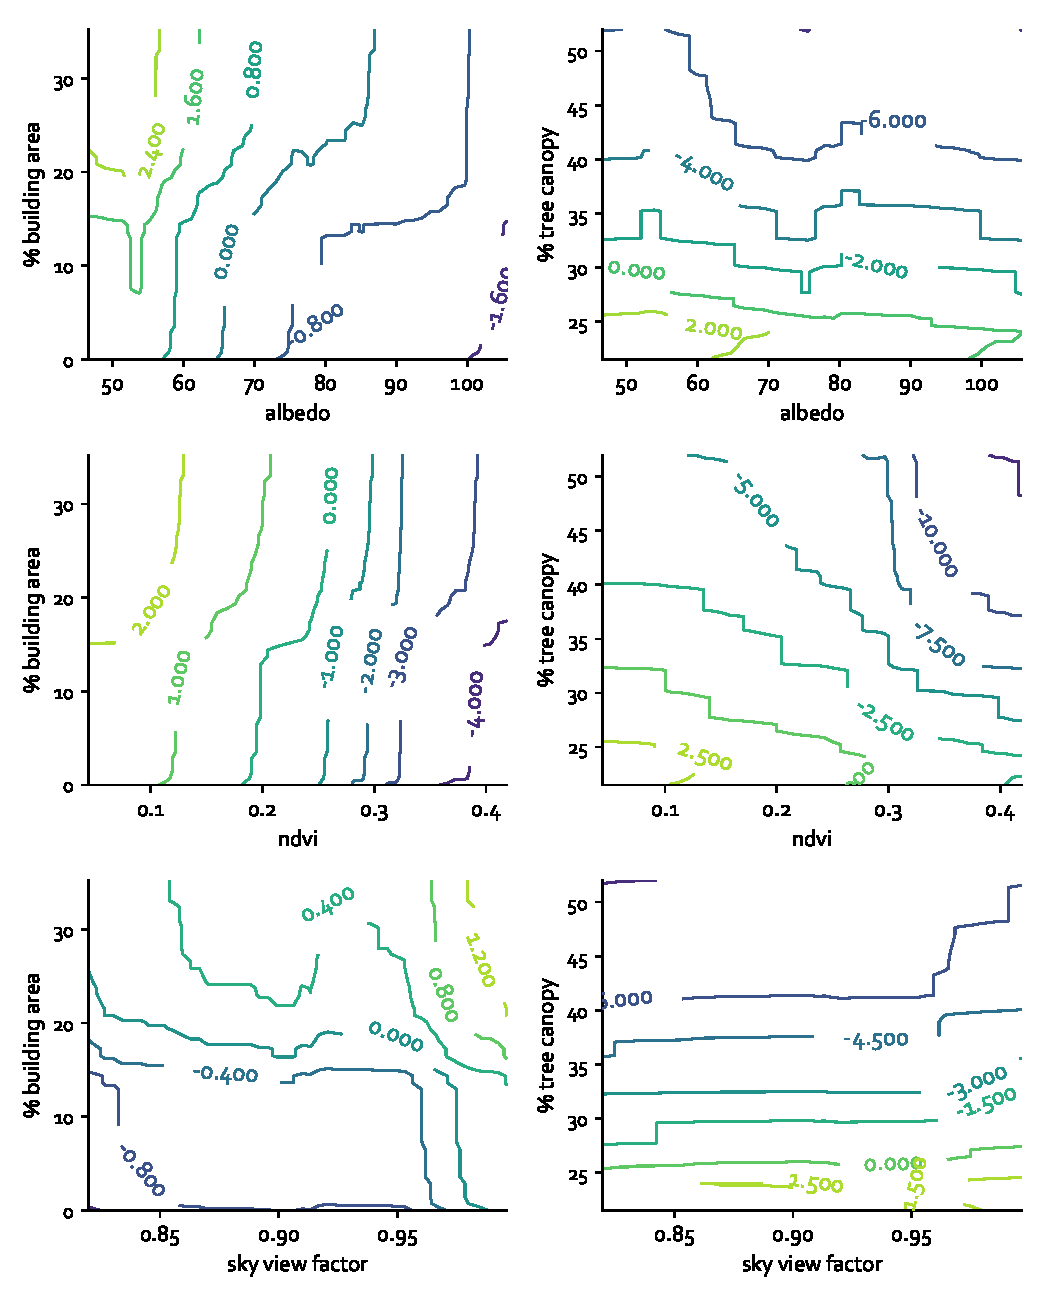
\includegraphics[width=\linewidth]{fig/report/pdp_2d_day_100.pdf}
    \caption{
    Partial dependence plots show how the land surface temperature ($^oC$, y axis) changes with each variable as the other variables are held at their average value. The left hand side shows the effect each variable has on LST during the night, while the right hand side shows the effect during the day. This shows that trees coverage in the cell has the greatest influence on the temperature, and the greenness (NDVI) of that coverage matters during the day.
    }
    \label{fig:pdp_2dday}
\end{figure}


\end{document}
